\documentclass[shadesubsections,compress,14pt,mathserif]{beamer}
\usepackage[danish]{babel}	
\usepackage{tikz}
\usetikzlibrary{shapes, positioning}
\usenavigationsymbolstemplate{}
\usepackage{pgfplots}
\usepackage[absolute,overlay]{textpos}
\usepackage{amsthm,amsfonts}
%\usepackage[T1]{fontenc}
% \usepackage{fullpage}
% Dokumentets sprog
%\usepackage{mathtools}
%\usepackage{pxfonts}
\usepackage{eulervm}
\usepackage[export]{adjustbox}
\everymath{\color{purple}}
% Class options include: notes, notesonly, handout, trans,
%                        hidesubsections, shadesubsections,
%                        inrow, blue, red, grey, brown

% Theme for beamer presentation.
%\usepackage{beamertheme} 
% Other themes include: beamerthemebars, beamerthemelined, 
%                       beamerthemetree, beamerthemetreebars  
\newcommand{\adv}{\ensuremath{\mathcal A}}
\newcommand{\F}{\ensuremath{{\mathbb F}}}
\newcommand{\Z}{\ensuremath{{\mathbb Z}}\xspace}
\newcommand{\Fclosure}{\ensuremath{{\overline{\mathbb{F}}}_p}}
\newcommand{\set}[1]{\ensuremath{\left\{#1\right\}}}
\newcommand{\sett}[2]{\ensuremath{\left\{#1\right\}_{#2}}}
\newcommand{\enc}[1]{\ensuremath{\left[#1\right ]}}
% \newcommand{\kzg}[1]{\ensuremath{\enc{#1(x)}}}
\newcommand{\cm}{\ensuremath{\mathsf{cm}}}
\newcommand{\kzg}[1]{\cm(#1)}
\newcommand{\open}[1]{\ensuremath{\mathsf{open}(#1)}}
\newcommand{\verify}[1]{\ensuremath{\mathsf{verify}(#1)}}
\newcommand{\defeq}{\ensuremath{:=}}
\newcommand{\helper}{\ensuremath{\mathcal{H}}}
\newcommand{\ver}{\ensuremath{\mathcal{V}}}
\newcommand{\prv}{\ensuremath{\mathcal{P}}}
 \newcommand{\polysofdeg}[1]{\F_{< #1}[X]}
%  \newcommand{\endoss}{\ensuremath{\mathrm{END}_E}}
 \newcommand{\hl}[1]{\textbf{\textit{#1}}}
 \newcommand{\polys}{\F[X]}
\newcommand{\acc}{{\mathbf{acc}}}
\newcommand{\ideal}{\mathbf{I}}
\newcommand{\gen}{\alpha}
\newcommand{\spac}{\\  \vspace{0.2in} \noindent}
\newcommand{\polylog}{\ensuremath{\mathsf{polylog}}\xspace}
% \renewcommand{\bf}{\begin{frame}}
% \newcommand{\ef}{\end{frame}}
%\setbeamersize{text margin left=3mm,text margin right=3mm}  
\newcommand{\nl}{\\ \pause \vspace{0.2in}}
\newcommand{\nlnp}{\\ \vspace{0.2in}}
\newcommand{\stitle}[1]{{\large{\textcolor{purple}{\emph{#1}}}}}
\DeclareMathAlphabet{\mathpgoth}{OT1}{pgoth}{m}{n}	
\newcommand{\cq}{\mathpgoth{cq} }
\newcommand{\cqstar}{\ensuremath{\mathpgoth{cq^{\mathbf{*}} }}\xspace}
\newcommand{\flookup}{\ensuremath{\mathsf{\mathpgoth{Flookup}}}\xspace}
\newcommand{\baloo}{\ensuremath{\mathrm{ba}\mathit{loo}}\xspace}
% \newcommand{\caulkp}{\ensuremath{\mathsf{\mathrel{Caulk}\mathrel{\scriptstyle{+}}}}\xspace}
\newcommand{\caulk}{\ensuremath{\mathsf{Caulk}}\xspace}
\newcommand{\plookup}{\ensuremath{\mathpgoth{plookup}}\xspace}
\newcommand{\srs}{\ensuremath{\mathsf{srs}}}
\newcommand{\tablegroup}{\ensuremath{\mathbb{H}}\xspace}
\newcommand{\V}{\ensuremath{\mathbf{V} }\xspace}
% \newcommand{\caulk}{{\mathsf{Caulk}}}
% \newcommand{\caulkp}{{\mathsf{\mathrel{Caulk}\mathrel{\scriptstyle{+}}}}}
\newcommand{\bigspace}{\ensuremath{\mathbb{V}}}
\newcommand{\papertitle}{Speeding up SNARKs with cached quotients}
%\newcommand{\authorname}}
\newcommand{\company}{}
\title{ \bf \papertitle \\[0.72cm]}
    \author{Ariel Gabizon} 

%\usefonttheme{professionalfonts}
%\usefonttheme[onlymath]{serif}
\begin{document}
\boldmath
% Creates title page of slide show using above information
\begin{frame}
  \titlepage
\end{frame}
                           % typeset with the notes or notesonly class options

%\section[Outline]{}

% Creates table of contents slide incorporating
% all \section and \subsection commands
\begin{frame}
\frametitle{The triology of pairing-based SNARKs}\pause

\begin{enumerate}
 \item \textbf{A new hope (for SNARKs, not the universe)} - [Groth10,\textbf{GGPR},...,Groth16]\pause 
 \vspace{0.2in}
 \item  \textbf{The polynomial commitment scheme strikes back} - [vsql,\textbf{Sonic},Plonk,Marlin,...]\pause 
 \vspace{0.2in}
 
 \item  \textbf{Return of the pairing} - [Caulk,...]
 
\end{enumerate}

\end{frame}
\begin{frame}
 \frametitle{First a short KZG Reminder..}   % Insert frame title between curly braces
 $\srs \defeq \enc{1},\enc{x},\ldots,\enc{x^d}$, for random $x\in \F$.\\ 
 $\cm(f)\defeq   \enc{f(x)}$\\ 
 \vspace{0.2in}
 Nice features:\pause
 \begin{itemize}
  \item \textbf{Linearity:} $\cm(f+g) = \cm(f)+\cm(g)$\pause
  \item \textbf{Product checks:} Given $\cm(f_1),\cm(f_2),\cm(g_1),\cm(g_2)$ can check $f_1(X)f_2(X)\stackrel{?}{\equiv} g_1(X)g_2(X)$ via pairings.\\
  (Secure in the Algebraic Group Model)
 \end{itemize}

\end{frame}

\begin{frame}
 \frametitle{ The first scene of chapter three from $\mathsf{Caulk}$}\pause
 $Z_T(X)=\prod_{a\in T} (X-a)$ 
 a vanishing polynomial of a subset $T\subset \F$.\nl
 $\cm(Z_T),\cm(f)$ given to verifier.\pause \\
 Prover wants to show $f=Z_S$ for some $S\subset T$.\pause
 \begin{figure}
  
\includegraphics[width=80pt]{jabba.png}
  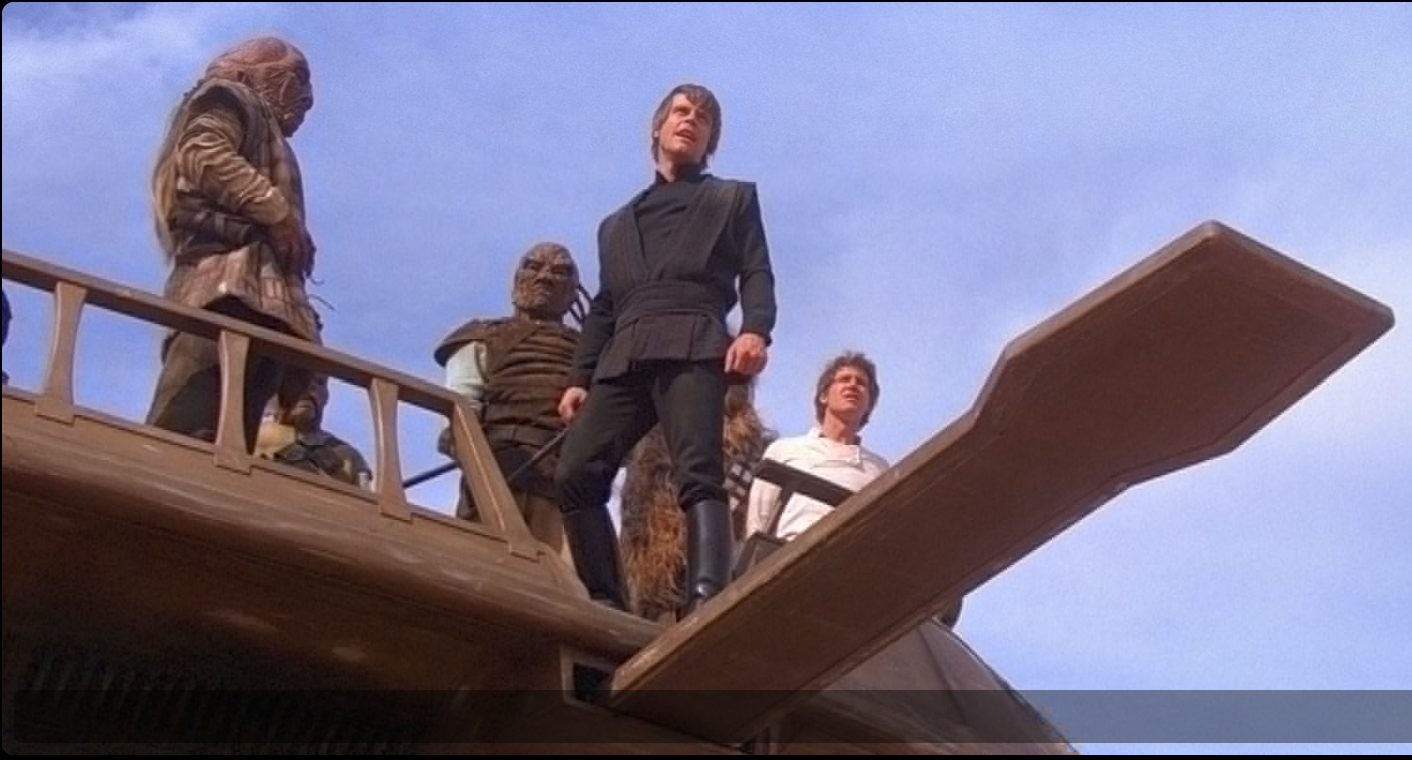
\includegraphics[width=120pt]{luke.png}
\end{figure}
 
 \textit{``Do it in  $O(|S|)$ prover operations or  be thrown in the pit!''} (think $|S|<<|T|$)
\end{frame}
\begin{frame}
 The quotient $Z_{T\setminus S}(X) =\frac{Z_T(X)}{Z_S(X)}$ is a ``witness'' to $S\subset T$. \nl
\begin{itemize}
 \item Enough to compute \textbf{commitment} to $Z_{T\setminus S}$. \pause
 \item This commitment is a \textbf{sparse combination} of commitments we can \textbf{precompute}.
\end{itemize}
\emph{details in next slide..}
\end{frame}

\begin{frame}
% \frametitle{Fractional decomposition:}
 For each $i\in T$, let $g_i(X)\defeq Z_{T\setminus\set{i}}(X)$.\nl
 We have {\small[Tomescu et. al]}
 \[\color{purple}Z_{T\setminus S} (X) = \sum_{i\in S} c_i\cdot g_i(X)\]
 for some $c_i\in \F$.\nl
 

 We precompute $\cm(Z_T),\sett{\cm(g_i)}{i\in T}$.\nlnp
\end{frame} 
 \begin{frame}
 Prover then computes in $|S|$ operations:
 \[\color{purple}\pi:=\cm(Z_{T\setminus S}) = \sum_{i\in S} c_i\cdot \cm(g_i)\]\nl
Verifier checks with pairing that:
\[\color{purple}e(\cm(f),\pi) =e(\cm(Z_T),\enc{1})\]
\end{frame}



 
\begin{frame}
 \frametitle{Sparse polynomials}
 parameters $n<<N$.\nl
 $B=\set{B_1(X),\ldots,B_N(X)}$ linearly independent set of polynomials.\nl
\textbf{Dfn:} $A\in \F[X]$  is \emph{$n$-sparse} in base $B$, if we can write
\[\color{purple} A(X)=\sum_{i\in [N]} a_i\cdot B_i(X)\]
where only $n$ $a_i$'s are non-zero.\nl

\emph{Default case:} $B$ is Lagrange base of subgroup of size $N$.
\end{frame}
% 
\begin{frame}
 \frametitle{Committing to sparse polynomials}
 We can precompute the KZG commitments for $B$:\\
$\srs_B \defeq \set{\kzg{B_1},\ldots,\kzg{B_N}}$\nl

Later, for $n$-sparse $A(X)$ we can compute 
\[\color{purple}\cm(A)=\sum_{i\in [N], a_i\neq 0} a_i\cdot \kzg{B_i}
\]
in $n$ operations. 
\end{frame}
\begin{frame}
 \frametitle{Cached quotients method}
 \textbf{Scenario:}
$T(X),Z(X)$ preprocessed polys. $\deg(Z)=N$.\nl
{\color{blue} Input:} $n$-sparse $A(X)$, and some $R(X)$ of deg$<N$.\\

$V$ has $\cm(A),\cm(R)$. \nl
Want to prove to $V$ that:
\[\color{purple}A(X)T(X)\equiv R(X) \; \mod\; Z(X)\]
 \textit{using $O(n)$ prover operations}.

\end{frame}
\begin{frame}
\frametitle{Cached quotients method}
There exists quotient $Q(X)$ such that $A\cdot T= Z\cdot Q+R$.\nl

We'll compute $\kzg{Q}$ in $n$ operations:\nl


\textbf{preprocessing:}
For each $i\in [N]$, compute $\kzg{Q_i}$ such that for some $R_i(X)\in \polysofdeg{N}$
\[\color{purple} B_i(X)\cdot T(X) = Q_i(X)\cdot Z(X) +R_i(X)\]\pause

Also precompute $\kzg{Z},\kzg{T}$
\end{frame}
\begin{frame}
\frametitle{$Q$ ``inherits'' $A$'s sparseness}
{\small \emph{$A(X)=\sum_{i} a_i B_i(X)$}}\\
After preprocessing, prover can compute and send
\[\color{purple} \kzg{Q}=\sum_{i\in [N],a_i\neq 0} a_i \cdot \kzg{Q_i}\]\nl
Verifier can then check with pairings:
\[\color{purple} AT\stackrel{?}{=}QZ+R\]
% \[\color{purple} e(\kzg{A},\kzg{T})=e(\kzg{Q},\kzg{Z})e(\kzg{R},\enc{1})\]
\end{frame}

    

\begin{frame}
\frametitle{Application  1: lookups }
Preprocessed table $T$ of size $N$, witness $f$ of size $n$, $n<<N$. Want to check $f_i\in T$ for each $i\in [n]$\nl 
{\color{blue} \small{[Caulk,...,$\cq$]}}: Can be done in  prover time $O(n\log n)$. \\
\emph{\small (improved plookup's $O(N\cdot \log N)$)}\nl
\textbf{proof sketch:} In log-derivative lookup {\color{blue} \small [Eagen,Hab{\"{o}}ck,..]} prover multiplies $n$-sparse poly with 
a preprocessed poly representing the table - \emph{good fit for cached quotients method.}
 
\end{frame}
\begin{frame}
\frametitle{Application 2: lincheck}
Fixed $n\times n$ matrix $M$.\nl
Prover has poly $f\in \polysofdeg{n}$.
Verifier $\cm(f)$.
$a\defeq f|_H$ for subgroup $H$ of size $n$.\nl

Prover wants to show $M\cdot a =0$
\emph{in $O(n)$ operations.}\nl

Let $L_1,\ldots,L_n$ be a Lagrange basis for $H$.


\end{frame}
\begin{frame}
 \frametitle{Reducing to cached quotients:}
 Represent $M$ by degree $\sim n^2$ polynomial
 \[\color{purple} M(X)\defeq \sum_{i,j \in [n]} M_{i,j} L_i(X^n)L_j(X)\]
Let $Z(X)\defeq X^{n^2}-1$.\nl
Let $A(X)\defeq f(X^n)$, $R\defeq A\cdot M \mod Z$.\nl
We have
\[\color{purple} R(X)=\sum_{j\in [n]}L_j(X) \sum_{i\in [n]} a_i\cdot M_{i,j}L_i(X^n).\]\pause
So $M\cdot a =0$ iff $R(X)\equiv 0 \mod X^n$.
% 
\end{frame}
\begin{frame}
Note that $A$ is $n$-sparse in the basis $\set{L_i(X^n)}$\nl
Use cached quotients twice to show
\begin{enumerate}
 \item 
 $A(X)\cdot M(X) \equiv R(X) \mod Z(X).$
 \item $R(X)\equiv 0 \mod X^n$.\nl
\end{enumerate}
\textit{Important point:} $R(X)$ is sparse in appropriate base of remainders in multiplication of $M$ modulu $Z$.
  
\end{frame}

\begin{frame}
\frametitle{Generalizing: The ``cached commitments methodology''}
 Given a polynomial IOP using prover poly $f$ that
 \begin{itemize}
  \item has high degree, but
  \item \emph{low sparsity} in a preknown basis of polynomials $B_1,\ldots,B_d$
  \item Is only used in degree$\leq 2$ verifier equations.
 \end{itemize}
 we can\pause
 \begin{enumerate}
  \item Precompure the KZG commitments to $B_1,\ldots,B_d$.
  \item In protocol time, only compute \emph{commitment} to $f$ from pre-computed commitments
  \item Use pairings to directly check verifier equations between commitments.
 \end{enumerate}
 \end{frame}
\end{document}
